\chapter{Design}

\section{Compiler Support}

There are several broad approaches to implementing an AOP framework. The ideal approach would be to extend the compiler of the target language to provide built-in support, thus making AOP the first class citizen. However there are very few languages out there that take this approach, among the few are Delphi Prism~\cite{delphi_prism2010} and AspectJ~\cite{aspectj_faq, aspectj_text}. 

Microsoft is currently in the "wait and see" mode regarding support of AOP development in the C\# compiler~\cite{hejlsberg}. Alternative compiler such as Mono C\#~\cite{monocsharp} is open source, so technically anyone can build AOP support into it. While that would have been a fun challenge, that would have been a fairly big undertaking, and there is concern that the project might not be finished in the time frame wanted.

That leaves framework support as the other viable option. There are several implementation techniques to provide AOP capabilities~\cite{aopcs, postsharp, aspectcs} via framework.

\section{Run-time Interception}

Early on the implementation approaches were narrowed down to between Run-time Interception and Compile Time Weaving. As its name suggested, run-time interception operates while the program is in execution. It uses the proxy pattern where client communicate with the target object via a proxy, and aspects are injected to the proxy. This enables run-time behavior of the program to be modified. Figure~\ref{proxy_model} illustrates this process.

\begin{figure}[H]
  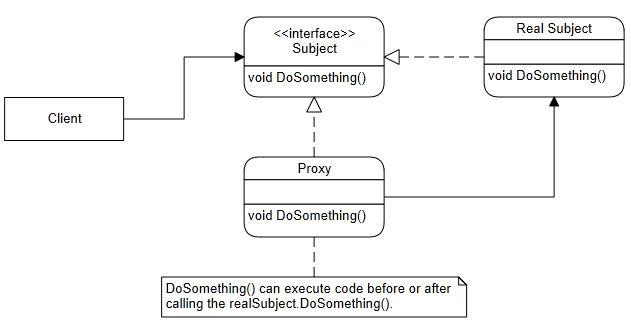
\includegraphics[scale=1.0]{Proxy3.PNG}
  \centering
  \caption{AOP Framework Using Proxy Pattern\label{proxy_model}}
\end{figure}

New functionality can be “added” to the target object via the proxy. The disadvantage of this approach is that it involves the generation of proxy object at run-time. The run-time performance of the application will be impacted as the result. It is also restricting in that both target object and the proxy must implement a common interface for this to work, and that only virtual methods are exposed for interception.

From the end user's perspective, to use it the developer usually have to provide some type of mapping between the target object and the proxy via a configuration file so the actual proxy generation can occur. This approach although is easier to implement, but not as easy and friendly to use. Buffalo is not taking this approach mainly because one of the goal is to be flexible and simple to use.

\section{Post Compilation Weaving}

The approach Buffalo takes is Post Compilation Weaving. The idea is that after compilation of the source code, the framework takes over and disassembles the assembly. Buffalo then weaves in the defined aspect code to all targeted methods. This approach is more difficult to implement as it involves modifying the underlying assembly by changing Common Intermediate Language (CIL) instructions~\cite{rewrite_msil}. But the advantage is that no run-time performance of proxy generation will be needed. 

Since injection happens post-compilation, the whole process can be integrated into the MS-Build system to have the weaving invoked automatically if needed. This will further reduce the steps needed from the developer.

Figure~\ref{buffalo_model} shows an overview of the compilation process and where Buffalo will fit in.

\begin{figure}[H]
  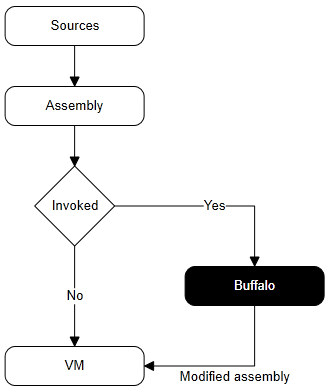
\includegraphics[scale=1.0]{BuffaloOverview2.PNG}
  \centering
  \caption{Buffalo Model\label{buffalo_model}}
\end{figure}

\section{A Buffalo Aspect}

When performing post compilation weaving, Buffalo has to be able to discover what aspect is applied to what methods in an assembly. In order to achieve that, the target assembly has to carry some identifying meta-data.

A given .NET assembly already carries a great deal of such meta-data for various purpose. .NET has the System.Attribute type that exists primarily for the purpose of inserting meta-data into the assembly during compilation. When the source code is compiled, it is converted into CIL~\cite{msil_text} and put inside a portable executable (PE) file, with the meta-data generated by the compiler. 

Buffalo takes advantage of this characteristic in two phases.
\begin{enumerate}
	\item An aspect defined in Buffalo will be in the form of an attribute, by sub-classing System.Attribute. It can contain any valid .NET code. But specifically an aspect needs to override various predefined methods in order to do something useful. The next section will discuss the relationship between various aspect types.
	\item After compilation, the assembly will now contain the meta-data about the aspect. Buffalo can inspect the assembly for the information, and perform CIL code injection accordingly.
\end{enumerate}

In other word, a Buffalo aspect is a .NET attribute in disguise.

\section{MethodBoundaryAspect}
What functionality does Buffalo support? What type of weaving does it do? For inspiration existing works such as AspectJ~\cite{aspectj_faq} and PostSharp~\cite{postsharp} were studied. Specifically Buffalo will intercept the various point of an executing method. Those points are namely: before a method executes; after a method executes; whether or not the method executed successfully without error; or whether the method throws an exception any point during the execution. These various points of interception are grouped into the MethodBoundaryAspect.

MethodBoundaryAspect can be cleanly mapped to the try-catch-finally statements of the .NET languages. As far as the runtime is concern~\cite{ecma334, ecma335}, try-catch can be used liberally without serious performance degradation. For example, a simple method shown in Figure~\ref{samplefunction}:

\begin{lstlisting}[caption={Sample function}, label=samplefunction]
public void SomeFunction () {
   //Perform some action...
}
\end{lstlisting}

The above can be transformed by Buffalo into something shown in Figure~\ref{sampletcf}. This clearly captures the spirit of the MethodBoundaryAspect. Regardless of whether the source already contain its own try-catch, or try-catch-finally blocks, the body of the method will be wrapped inside of a new try-catch-finally block by Buffalo.

\begin{lstlisting}[caption={Sample try-catch-finally}, label=sampletcf]
public void SomeFunction () {
   try {
       OnBefore();
       //Perform some action
       OnSuccess();
   }
   catch (Exception e) {
       OnException(e);
   }
   finally {
       OnAfter();
   }
}
\end{lstlisting}

Transformed method in Figure~\ref{sampletcf} still does what the original method intends to do, only now at various point execution are being intercepted to provide more functionality. 

\section{MethodAroundAspect}
Another type of aspect that Buffalo supports is the MethodAroundAspect. Rather than intercepting various execution points of a method, the method can be completely replaced by another method defined in an aspect, while preserving the option to call back into the original method if necessary.

At first glance MethodAroundAspect sounds straightforward to do, but it turns out to be much more involved than the MethodBoundaryAspect.

Since the option to call back into the original method is preserved, it is critical that under no circumstance should the original method be modified. If the method body instructions are simply overridden with that of the replacement, the call back to the original method will be meaningless since the method is now changed. The original method must be intact for the call back to happen.

To get around this obstacle, whenever Buffalo encounters the MethodAroundAspect applied to a method, it dynamically generates a replacement method in CIL with the same method signature as the original.

The body of this replacement method is also completely different than the original. It instantiates the aspect and makes call to the Invoke() method, which is the actual code that will be ran as a replacement. 

Inside the Invoke method, developer can make a call back to the original method via a call to the Proceed() method. Then throughout the program, for any calls made to the original method, Buffalo would change them to call the replacement method instead. This is illustrated in figure~\ref{around_overview}.

\begin{figure}[H]
  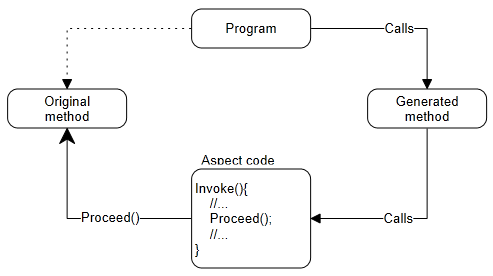
\includegraphics[scale=1.0]{AroundOverview3.PNG}
  \centering
  \caption{Overview of MethodAroundAspect\label{around_overview}}
\end{figure}

The dotted line from Program to the Original method indicates that once the MethodAroundAspect is applied to it, from the perspective of CIL the program cannot directly access that method any more. Access to the original method now has to come from inside the aspect. Also note that the original method is not changed at any given time.
